The missing transverse energy (\met) trigger is an essential trigger for numerous physics searches in ATLAS, including two searches led by UTA:  the search for an invisible Higgs in the Vector Boson Fusion production mode; and the search for a charged Higgs decaying to a tau lepton and its associated neutrino.   The \met\ trigger is preferable in the invisible Higgs search due to the high rates of forward jets, and the relatively low efficiency of a pure VBF trigger studies are ongoing on the feasibility of combining VBF and \met\ topologies with use of the L1Topo         (topological processor).  On the other hand the \met\ trigger is preferred over tau or multi-jet triggers in the H$^+ \Rightarrow\tau\nu$ search due to inefficiencies in the tau triggers and the bias a tau trigger introduces in the data driven background estimation techniques.

For a \met\ only trigger to be effective for searches it should remain unprescaled.
For the 2016 data taking period a trigger with $\met> 50$ GeV at the hardware trigger level (L1) is effective at controlling the rate into the high level trigger (HLT), and it was envisioned that a requirement of at least 80 GeV on the vector sum of topological clusters would be sufficient to control the rates out of the HLT for the entire year. It became clear after a few months of data taking that the trigger rate growth with increased luminosity would soon be unsustainable.   UTA Graduate Student, Last Feremenga, studied the feasibility of maintaining the cluster based \met\ triggers by recalculating the vector sum without forward clusters, which might be more susceptible to multiple interactions He showed that while efficiency was unaffected by restricting the cluster eta position, the rates were also largely unchanged.  A trigger which replaced the cluster sum of 80 with a sum of the jets 
$ met>90 GeV$, was better behaved, but the excellent performance of the LHC necessitated an increase in threshold to 110 GeV for the ICHEP data set.  As of September 2016, it was decided that this trigger would not be tenable for the rest of the run. Rather than raise the threshold again, our efficiency studies indicated that it was better to add a requirement on the vector sum of all cells above noise threshold,.


\begin{figure}[htb]
\centering
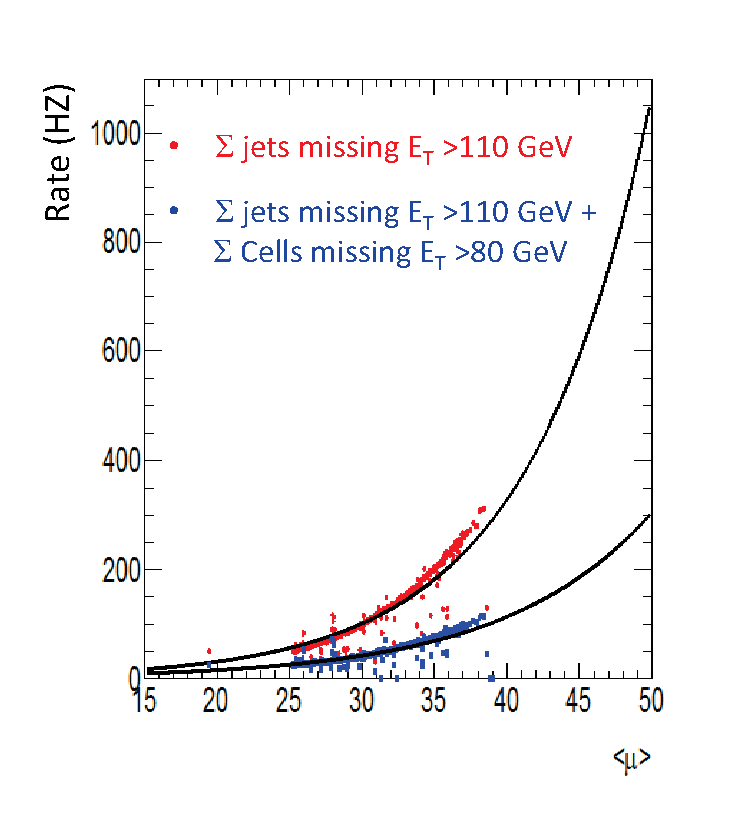
\includegraphics[height=3in, width=0.50\textwidth]{images/met-growth-labc.eps}
\caption[]{Rates vs $<\mu>$ for the 110 GeV jet sum with (blue) and without (red) the additional requirement that the vector sum of the cells is greater than 70 GeV.}
\label{fig:mettrigger}
\end{figure}  


This solution lowers the rate sufficiently for the 2016 data taking, but as seen in Figure 1, the exponential rate dependence on  $<\mu>$ remains.  

The understanding of the \met\ trigger rates will remain a high priority for many analyses moving forward in 2017 and beyond as the pileup conditions at the LHC become more intense.  We plan to help fully understand the issue and devise longer-term solutions.  Based on our previous trigger experience with forward jets, pileup, and topology tools, we have several ideas to help develop a longer term solution improve. Some potential improvements include:   adding a minimum \pt\ requirement on jets that go into the vector sum, placing a minimum \pt\ requirement on the leading jet in the event, ensuring the leading jet is not collinear with the \met, suppression of pileup jets using FTK tracks in conjunction with the offline JVT algorithm, etc. 
